\documentclass{standalone}
\usepackage{tikz}
\usepackage{adjustbox}
\usepackage{helvet}  
\usepackage{sansmathfonts}  
\renewcommand{\familydefault}{\sfdefault}  
\usetikzlibrary{arrows.meta,calc,decorations.pathmorphing}
\usetikzlibrary{shapes.geometric, shapes.arrows}
\usepackage{xcolor}

\definecolor{color0000FF}{HTML}{0000FF}
\definecolor{colorADD8E6}{HTML}{ADD8E6}
\definecolor{colorFF0000}{HTML}{FF0000}
\definecolor{colorFFC0CB}{HTML}{FFC0CB}
\definecolor{color008000}{HTML}{008000}
\definecolor{color90EE90}{HTML}{90EE90}
\definecolor{colorFFA500}{HTML}{FFA500}
\definecolor{colorFFFF00}{HTML}{FFFF00}
\definecolor{color800080}{HTML}{800080}
\definecolor{colorE6E6FA}{HTML}{E6E6FA}
\definecolor{color000000}{HTML}{000000}
\definecolor{colorD3D3D3}{HTML}{D3D3D3}
\begin{document}
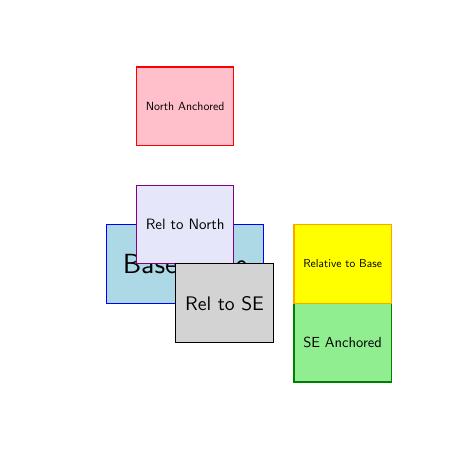
\begin{tikzpicture}
\useasboundingbox (1,1) rectangle (6,6);



\node[draw=color0000FF, fill=colorADD8E6, minimum width=2cm, minimum height=1cm] (base) at (3,3) {\adjustbox{max width=2cm, max height=1cm}{Base Node}};
\node[draw=colorFF0000, fill=colorFFC0CB, minimum width=1cm, minimum height=1cm] (north_anchored) at (3,5) {\adjustbox{max width=1cm, max height=1cm}{North Anchored}};
\node[draw=color008000, fill=color90EE90, minimum width=1cm, minimum height=1cm] (south_east_anchored) at (5,2) {\adjustbox{max width=1cm, max height=1cm}{SE Anchored}};
\node[draw=colorFFA500, fill=colorFFFF00, minimum width=1cm, minimum height=1cm] (rel_to_base) at (5,3) {\adjustbox{max width=1cm, max height=1cm}{Relative to Base}};
\node[draw=color800080, fill=colorE6E6FA, minimum width=1cm, minimum height=1cm] (rel_to_north) at (3,3.5) {\adjustbox{max width=1cm, max height=1cm}{Rel to North}};
\node[draw=color000000, fill=colorD3D3D3, minimum width=1cm, minimum height=1cm] (rel_to_se) at (3.5,2.5) {\adjustbox{max width=1cm, max height=1cm}{Rel to SE}};

\end{tikzpicture}
\end{document}